\documentclass[a4paper]{article}
\usepackage[utf8x]{inputenc}
\usepackage[T1,T2A]{fontenc}
\usepackage[russian]{babel}
\usepackage{hyperref}
\usepackage{indentfirst}
\usepackage{listings}
\usepackage{color}
\usepackage{here}
\usepackage{array}
\usepackage{multirow}
\usepackage{graphicx}
\usepackage{caption}
\graphicspath{{graphics/}}
\usepackage[left=2cm,right=2cm,
top=2cm,bottom=2cm,bindingoffset=0cm]{geometry}
\usepackage{listings}
\lstset{ %
	extendedchars=\true,
	keepspaces=true,
	language=bash,					% choose the language of the code
	basicstyle=\footnotesize,		% the size of the fonts that are used for the code
	numbers=left,					% where to put the line-numbers
	numberstyle=\footnotesize,		% the size of the fonts that are used for the line-numbers
	stepnumber=1,					% the step between two line-numbers. If it is 1 each line will be numbered
	numbersep=5pt,					% how far the line-numbers are from the code
	backgroundcolor=\color{white},	% choose the background color. You must add \usepackage{color}
	showspaces=false				% show spaces adding particular underscores
	showstringspaces=false,			% underline spaces within strings
	showtabs=false,					% show tabs within strings adding particular underscores
	frame=single,           		% adds a frame around the code
	tabsize=2,						% sets default tabsize to 2 spaces
	captionpos=b,					% sets the caption-position to bottom
	breaklines=true,				% sets automatic line breaking
	breakatwhitespace=false,		% sets if automatic breaks should only happen at whitespace
	escapeinside={\%*}{*)},			% if you want to add a comment within your code
	postbreak=\raisebox{0ex}[0ex][0ex]{\ensuremath{\color{red}\hookrightarrow\space}}
}

\begin{document}	% начало документа

\begin{titlepage}	% начало титульной страницы

	\begin{center}		% выравнивание по центру

		\large Санкт-Петербургский Политехнический Университет Петра Великого\\
		\large Институт компьютерных наук и технологий \\
		\large Кафедра компьютерных систем и программных технологий\\[6cm]
		% название института, затем отступ 6см
		
		\huge Телекоммуникационные технологии\\[0.5cm] % название работы, затем отступ 0,5см
		\large Отчет по лабораторной работе №7 \\[0.2cm]
		\large\textbf{"Помехоустойчивое кодирование
"}\\[5cm]

	\end{center}


	\begin{flushright} % выравнивание по правому краю
		\begin{minipage}{0.25\textwidth} % врезка в половину ширины текста
			\begin{flushleft} % выровнять её содержимое по левому краю

				\large\textbf{Работу выполнила:}\\
				\large Власова А.В.\\
				\large {Группа:} 33501/4\\
				
				\large \textbf{Преподаватель:}\\
				\large Богач Н.В.\

			\end{flushleft}
		\end{minipage}
	\end{flushright}
	
	\vfill % заполнить всё доступное ниже пространство

	\begin{center}
	\large Санкт-Петербург\\
	\large \the\year % вывести дату
	\end{center} % закончить выравнивание по центру

\thispagestyle{empty} % не нумеровать страницу
\end{titlepage} % конец титульной страницы

\vfill % заполнить всё доступное ниже пространство

\section{Цель работы}
Изучение методов помехоустойчивого кодирования и сравнение их свойств.

\section{Постановка задачи}
\begin{itemize}
	\item Провести кодирование/декодирование сигнала, полученного с помощью функции randerr кодом Хэмминга 2-мя способами: с помощью встроенных функций encode/decode, а также через	создание проверочной и генераторной матриц и вычисление синдрома. Оценить корректирующую способность кода.
	\item Выполнить кодирование/декодирование циклическим кодом, кодом БЧХ, кодом Рида-Соломона. Оценить корректирующую способность кода.
\end{itemize}


\section{Теоретический раздел}
Кодирование информации — процесс преобразования сигнала из формы, удобной для непосредственного использования информации, в форму, удобную для передачи, хранения или автоматической переработки.\\

Коды можно разделить на две самостоятельные группы. К первой относятся коды, использующие все возможные комбинации – неизбыточные коды. Ко второй группе относятся коды, использующие лишь определенную часть всех возможных комбинаций, такие коды называются избыточными. Оставшаяся часть комбинаций используется для обнаружения или исправления ошибок, возникающих при передаче сообщений. В этих кодах количество разрядов кодовых комбинаций можно условно разделить на определенное число разрядов, предназначенных для информации (информационные разряды), и число разрядов, предназначенных для коррекции ошибок (проверочные разряды).\\

Все корректирующие (избыточные) коды делятся на два больших класса: блочные и непрерывные коды. При кодировании блочным кодом последовательность $k$ элементов данных от источника сообщений принимается за блок (сообщение). Каждому возможному блоку из $k$ информационных символов ставится в соответствие кодовый блок (слово) длиной $n$. Код называется $(n,k)$- кодом. Кодовый блок в канале связи искажается шумом и декодируется независимо от других кодовых блоков.\\

Разделимые блочные коды, в свою очередь, делятся на несистематические и систематические.Основная особенность систематических кодов в том, что проверочные символы в них образуются как линейные комбинации информационных символов.\\

Разновидностью систематических кодов являются циклические коды. Циклические коды имеют следующее свойство: если некоторая кодовая комбинация принадлежит коду, то получающаяся путем циклической перестановки символов новая комбинация также принадлежит данному коду. К наиболее известным циклическим кодам относятся простейшие коды, коды Хэмминга, Боуза-Чоудхури-Хоквингема, мажоритарные, Рида-Соломона и др.
 
\section{Ход работы}
Выполним кодирование/декодирование посылки кодом Хэмминга с помощью функций encode/decode.

\captionof{lstlisting}{Кодирование с помощью encode/decode}
\lstinputlisting[firstline=4, lastline=8]{../lab7.m}

Результаты работы программы: \\
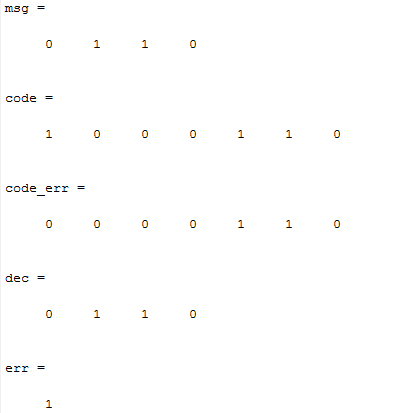
\includegraphics[scale = 0.7]{res1.png}

Выполним кодирование/декодирование через создание проверочной и генераторной матриц и вычисление синдрома.

\captionof{lstlisting}{Кодирование с помощью матриц}
\lstinputlisting[firstline=10, lastline=20]{../lab7.m}

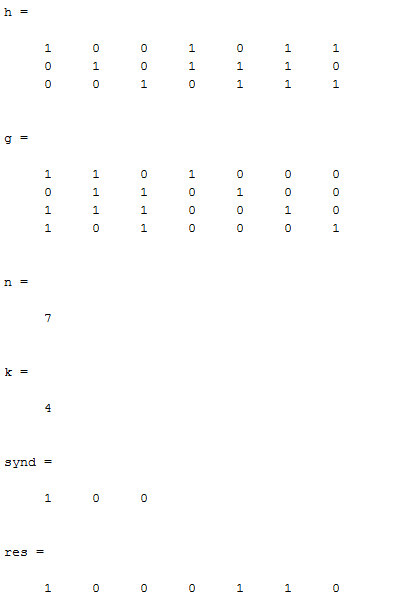
\includegraphics[scale = 0.7]{res2.png}

Выполним кодирование/декодирование циклическим кодом.
\captionof{lstlisting}{Кодирование циклическим кодом}
\lstinputlisting[firstline=22, lastline=34]{../lab7.m}

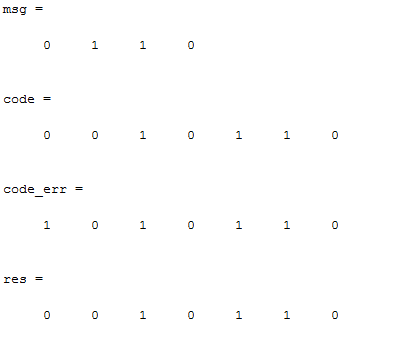
\includegraphics[scale = 0.7]{res3.png}

Выполним кодирование/декодирование кодом БЧХ.
\captionof{lstlisting}{Кодирование кодом БЧХ}
\lstinputlisting[firstline=36, lastline=43]{../lab7.m}

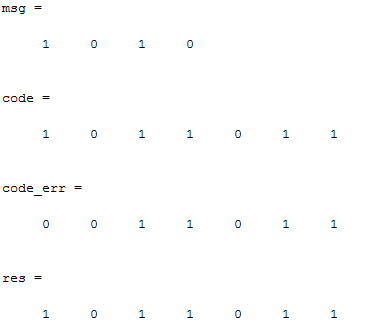
\includegraphics[scale = 0.7]{res4.png}

Выполним кодирование/декодирование кодом Рида-Соломона.
\captionof{lstlisting}{Кодирование кодом Рида-Соломона}
\lstinputlisting[firstline=45, lastline=51]{../lab7.m}

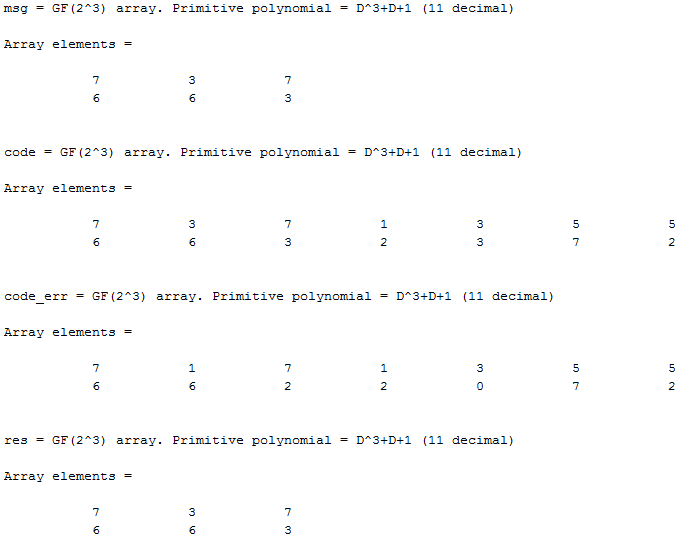
\includegraphics[scale = 0.7]{res5.png}

\section{Выводы}
В ходе выполнения лабораторной работы выполнено кодирование/декодирование посылок с применением разного вида кода. Корректирующая способность кодов БЧХ и Рида-Соломона выше корректирующей способности кода Хэмминга и циклического кода.
\end{document}



